\chapter{Elementen in het heelal en op aarde}\label{ch:g9:elements-universe-earth}

Het calcium in je botten, het ijzer in je bloed en de zuurstof die je
inademt, zijn niet op aarde gemaakt. Ze zijn gemaakt in sterren die
leefden en stierven voordat de zon geboren werd, en al miljarden jaren
gaan ze over van gesteente naar zee, van zee naar plant, van plant naar
dier. Sommige elementen zijn overal, andere zeldzaam. Uit welke
elementen bestaan de sterren, de aarde, de oceanen --- en wijzelf?

\begin{recall}
Een \omterm{def:g9:inside-the-atom:element}{chemisch element} is de verzameling \omterm{def:g7:atoms-and-molecules:atom}{atomen} met hetzelfde \omterm{def:g9:inside-the-atom:atomic-number}{atoomnummer}
$Z$; de massa van een \omterm{def:g7:atoms-and-molecules:atom}{atoom} ligt dicht bij $A \times \qty{1.67e-27}{kg}$,
waarbij $A$ het \omterm{def:g9:inside-the-atom:atomic-number}{massagetal} is (\cref{ch:g9:inside-the-atom}). Het
\omterm{def:g9:periodic-table-first-look:periodic-table}{periodiek systeem} zet de 118 elementen op volgorde van \omterm{def:g9:inside-the-atom:atomic-number}{atoomnummer}
(\cref{ch:g9:periodic-table-first-look}). \omterm{def:g4:air-a-mixture-of-gases:air}{Lucht} bestaat voor ongeveer
vier vijfde uit stikstof en voor een vijfde uit zuurstof
(\cref{ch:g4:air-a-mixture-of-gases}).
\end{recall}

\section{De elementen van de sterren}

\begin{definition}[Abundantie]\label{def:g9:elements-universe-earth:abundance}
De \emph{abundantie}\index{abundantie} van een element in een
hoeveelheid materie --- een ster, de aardkorst, de oceaan, een levend
wezen --- is zijn aandeel in de totale massa, meestal gegeven in
procent.
\end{definition}

\begin{proposition}[De zon is waterstof en helium]\label{prop:g9:elements-universe-earth:sun}
% ledger: ab:sun-X, ab:sun-Y, ab:sun-Z
Het oppervlak van de zon bestaat in massa voor ongeveer
\qty{74}{\percent} uit waterstof en voor \qty{25}{\percent} uit helium;
alle andere elementen samen maken maar ongeveer \qty{1.3}{\percent} uit.
Het grootste deel van de zichtbare materie in het heelal heeft een
vergelijkbare samenstelling: waterstof en helium, met een snufje van al
het andere.
\end{proposition}

\begin{proposition}[Elementen gemaakt in sterren]\label{prop:g9:elements-universe-earth:stars}
Waterstof en het meeste helium zijn in de eerste minuten van het heelal
ontstaan. Bijna alle zwaardere elementen --- koolstof, zuurstof, ijzer,
goud --- zijn later gemaakt, binnen in sterren, en in de ruimte
verspreid toen sterren ontploften. Uit dat verrijkte stof ontstonden
nieuwe sterren en planeten. Hoe de sterren dat doen, staat in het
natuurkundeboek.
\end{proposition}

\begin{omfigure}
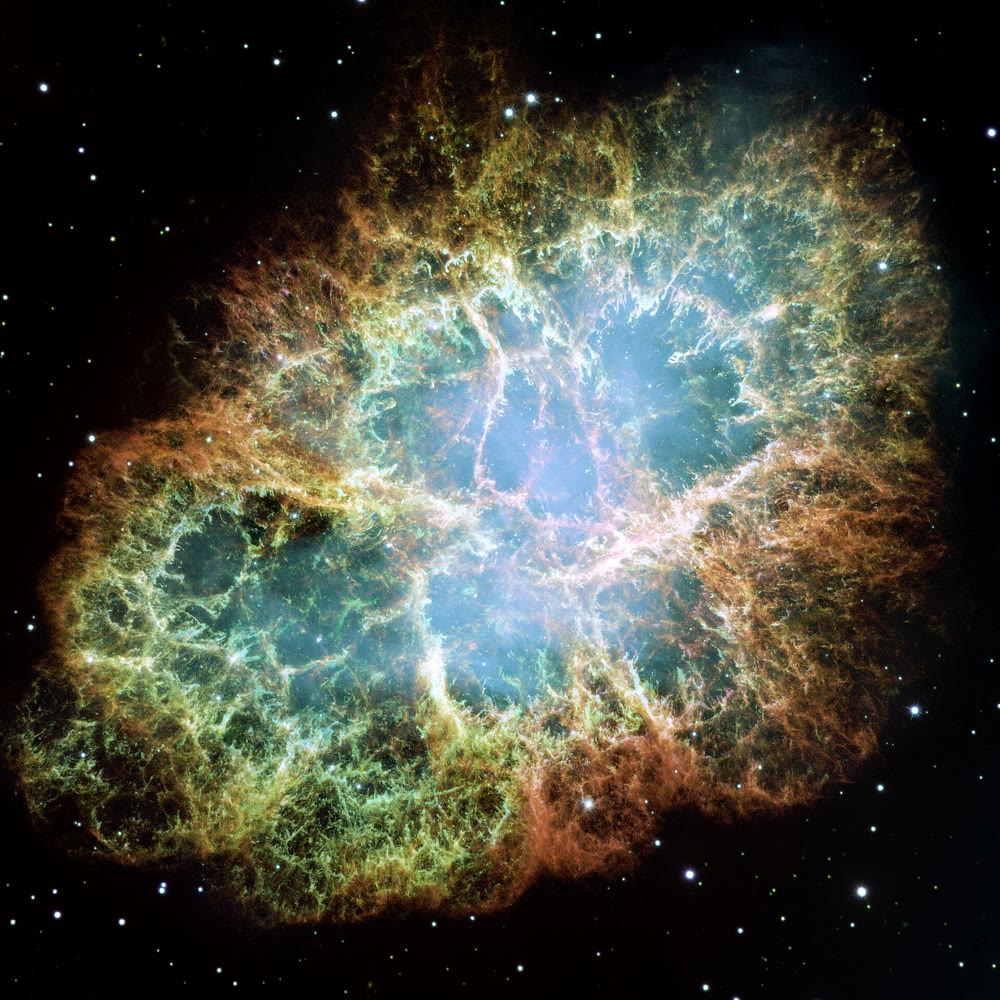
\includegraphics[width=0.45\linewidth]{images/book1/crab-nebula.jpg}

{\small De Krabnevel, de wolk die een ster achterliet die bijna duizend
jaar geleden ontplofte, en die nieuwe elementen in de ruimte verspreidt
(NASA, ESA, J.~Hester en A.~Loll).}
\end{omfigure}

\section{De aarde}

\begin{proposition}[De aardkorst]\label{prop:g9:elements-universe-earth:crust}
% ledger: ab:crust-O, ab:crust-Si, ab:crust-Al, ab:crust-Fe, ab:crust-Ca, ab:crust-Na, ab:crust-K, ab:crust-Mg, ab:crust-first10
De dunne stenen huid van de aarde, de aardkorst, bestaat in massa voor
bijna de helft uit zuurstof en voor meer dan een kwart uit silicium:
gesteenten en zand zijn vooral oxiden van silicium en van een paar
\omterm{def:g9:periodic-table-first-look:metal}{metalen}. Acht elementen --- zuurstof, silicium, aluminium, ijzer,
calcium, natrium, kalium, magnesium --- vormen er samen ongeveer
\qty{99}{\percent} van. Waterstof en helium, zo gewoon in de sterren,
zijn er zeldzaam: de lichte gassen zijn uit de jonge aarde ontsnapt.
\end{proposition}

\begin{remark}[Binnen in de aarde]\label{rem:g9:elements-universe-earth:core}
De aardkorst is niet de hele aarde. IJzer, dat zwaar is, zakte naar het
midden toen de jonge aarde gesmolten was: de kern van de aarde bestaat
vooral uit ijzer, met wat nikkel.
\end{remark}

\begin{proposition}[De oceanen en de lucht]\label{prop:g9:elements-universe-earth:ocean}
% ledger: sea:salts-share, sea:NaCl-ions, sea:MgSO4-ions, air:N2, air:O2
Zeewater is vooral water --- waterstof en zuurstof --- met ongeveer
\qty{3.5}{\percent} opgeloste zouten in massa. Van de opgeloste \omterm{def:g9:ions:ion}{ionen}
zijn chloride en natrium samen ongeveer \qty{85}{\percent}, magnesium en
sulfaat nog eens \qty{10}{\percent}. De \omterm{def:g4:air-a-mixture-of-gases:air}{lucht} is vooral stikstof en
zuurstof.
\end{proposition}

\begin{omfigure}
\begin{tikzpicture}
\begin{axis}[xbar, width=0.40\linewidth, height=5.4cm, xmin=0, xmax=85,
    bar width=7pt, symbolic y coords={Mg,K,Na,Ca,Fe,Al,Si,O}, ytick=data,
    xlabel={procent van de massa}, title={\small de aardkorst},
    nodes near coords, nodes near coords style={font=\scriptsize},
    tick label style={font=\small}, label style={font=\small},
    axis lines*=left, enlarge y limits=0.08]
% ledger: ab:crust-O, ab:crust-Si, ab:crust-Al, ab:crust-Fe, ab:crust-Ca, ab:crust-Na, ab:crust-K, ab:crust-Mg
\addplot[fill=omDef!45, draw=omDef] coordinates {(46.6,O) (27.7,Si) (8.1,Al)
  (5.0,Fe) (3.6,Ca) (2.8,Na) (2.6,K) (2.1,Mg)};
\end{axis}
\end{tikzpicture}\hfill
\begin{tikzpicture}
\begin{axis}[xbar, width=0.40\linewidth, height=5.4cm, xmin=0, xmax=85,
    bar width=7pt, symbolic y coords={{P},{N},{Ca},{H},{C},{O}}, ytick=data,
    xlabel={procent van de massa}, title={\small een menselijk lichaam},
    nodes near coords, nodes near coords style={font=\scriptsize},
    tick label style={font=\small}, label style={font=\small},
    axis lines*=left, enlarge y limits=0.1]
% ledger: body:atoms-O, body:atoms-C, body:atoms-H, body:atoms-N, body:atoms-Ca, body:atoms-P (masses = atoms x atomic mass, over 70 kg)
\addplot[fill=omProp!45, draw=omProp] coordinates {(61.1,O) (22.9,C) (10.1,H)
  (1.3,N) (1.5,Ca) (0.7,P)};
\end{axis}
\end{tikzpicture}

{\small \omterm{def:g9:elements-universe-earth:abundance}{Abundanties} in massa. Links: de acht belangrijkste elementen van
de aardkorst. Rechts: de zes belangrijkste elementen van een slank
volwassen menselijk lichaam (berekend uit geschatte aantallen \omterm{def:g7:atoms-and-molecules:atom}{atomen}).}
\end{omfigure}

\section{Het menselijk lichaam}

\begin{proposition}[Waar we van gemaakt zijn]\label{prop:g9:elements-universe-earth:body}
% ledger: body:atoms-O, body:atoms-C, body:atoms-H, body:atoms-N, body:atoms-Ca, body:atoms-P, body:atoms-total
In massa bestaat een slank volwassen lichaam voor ongeveer
\qty{61}{\percent} uit zuurstof, \qty{23}{\percent} uit koolstof en
\qty{10}{\percent} uit waterstof --- vooral in water en in de \omterm{def:g7:atoms-and-molecules:molecule}{moleculen}
van het leven --- gevolgd door stikstof, calcium (in botten en tanden)
en fosfor. Tel je in \omterm{def:g7:atoms-and-molecules:atom}{atomen} in plaats van in massa, dan verandert de
volgorde: er zitten meer waterstofatomen in een lichaam dan alle andere
\omterm{def:g7:atoms-and-molecules:atom}{atomen} samen, omdat waterstofatomen zo licht zijn. Een lichaam van
\qty{70}{kg} bevat ongeveer $7 \times 10^{27}$ \omterm{def:g7:atoms-and-molecules:atom}{atomen}.
\end{proposition}

\begin{method}[Een abundantiediagram lezen]\label{met:g9:elements-universe-earth:read}
\begin{enumerate}
  \item Kijk wat er gemeten is: massa (de meeste diagrammen) of aantal
        \omterm{def:g7:atoms-and-molecules:atom}{atomen}.
  \item Lees het aandeel van elk element af; tel die van de belangrijkste
        op om te zien hoeveel ze samen beslaan.
  \item Om twee lichamen te vergelijken, zoek je de elementen die in
        beide voorkomen en die welke in maar één voorkomen.
\end{enumerate}
Zuurstof staat in beide diagrammen van dit hoofdstuk bovenaan: het is
het meest voorkomende element van de aardkorst en van het menselijk
lichaam, in massa.
\end{method}

\section{Dezelfde atomen, steeds opnieuw gebruikt}

\begin{example}[De reis van een koolstofatoom]\label{ex:g9:elements-universe-earth:journey}
Een koolstofatoom dat lang geleden in een ster is gemaakt, kan miljoenen
jaren in kalksteen zitten, door een vulkaan als koolstofdioxide
vrijkomen, door een blad worden opgenomen, deel worden van een suiker in
een vrucht, terechtkomen in een dier dat de vrucht opeet, en weer als
koolstofdioxide worden uitgeademd. \omterm{def:g7:atoms-and-molecules:atom}{Atomen} worden door \omterm{def:g5:irreversible-changes:chemical-change}{chemische
veranderingen} niet vernietigd: ze worden doorgegeven.
\end{example}

\begin{omfigure}
\begin{tikzpicture}[font=\small,
    box/.style={draw=omDef, fill=omDef!6, rounded corners=2pt, align=center,
      minimum height=0.85cm, text width=2.3cm}]
  \node[box] (a) at (0,2.2) {in een gesteente\\ (kalksteen)};
  \node[box] (b) at (4.3,2.2) {in de lucht\\ (\ce{CO2})};
  \node[box] (c) at (8.6,2.2) {in een blad\\ (suiker)};
  \node[box] (d) at (8.6,0) {in een dier};
  \node[box] (e) at (4.3,0) {uitgeademd\\ (\ce{CO2})};
  \draw[->, thick, omProp] (a) -- node[above, font=\footnotesize] {vulkaan} (b);
  \draw[->, thick, omProp] (b) -- (c);
  \draw[->, thick, omProp] (c) -- node[right, font=\footnotesize] {opgegeten} (d);
  \draw[->, thick, omProp] (d) -- (e);
  \draw[->, thick, omProp] (e) -- (b);
\end{tikzpicture}

{\small Een koolstofatoom gaat van gesteente naar \omterm{def:g4:air-a-mixture-of-gases:air}{lucht} naar blad naar
dier en weer terug naar de \omterm{def:g4:air-a-mixture-of-gases:air}{lucht}: het \omterm{def:g7:atoms-and-molecules:atom}{atoom} zelf wordt nooit
vernietigd.}
\end{omfigure}

\begin{omfigure}
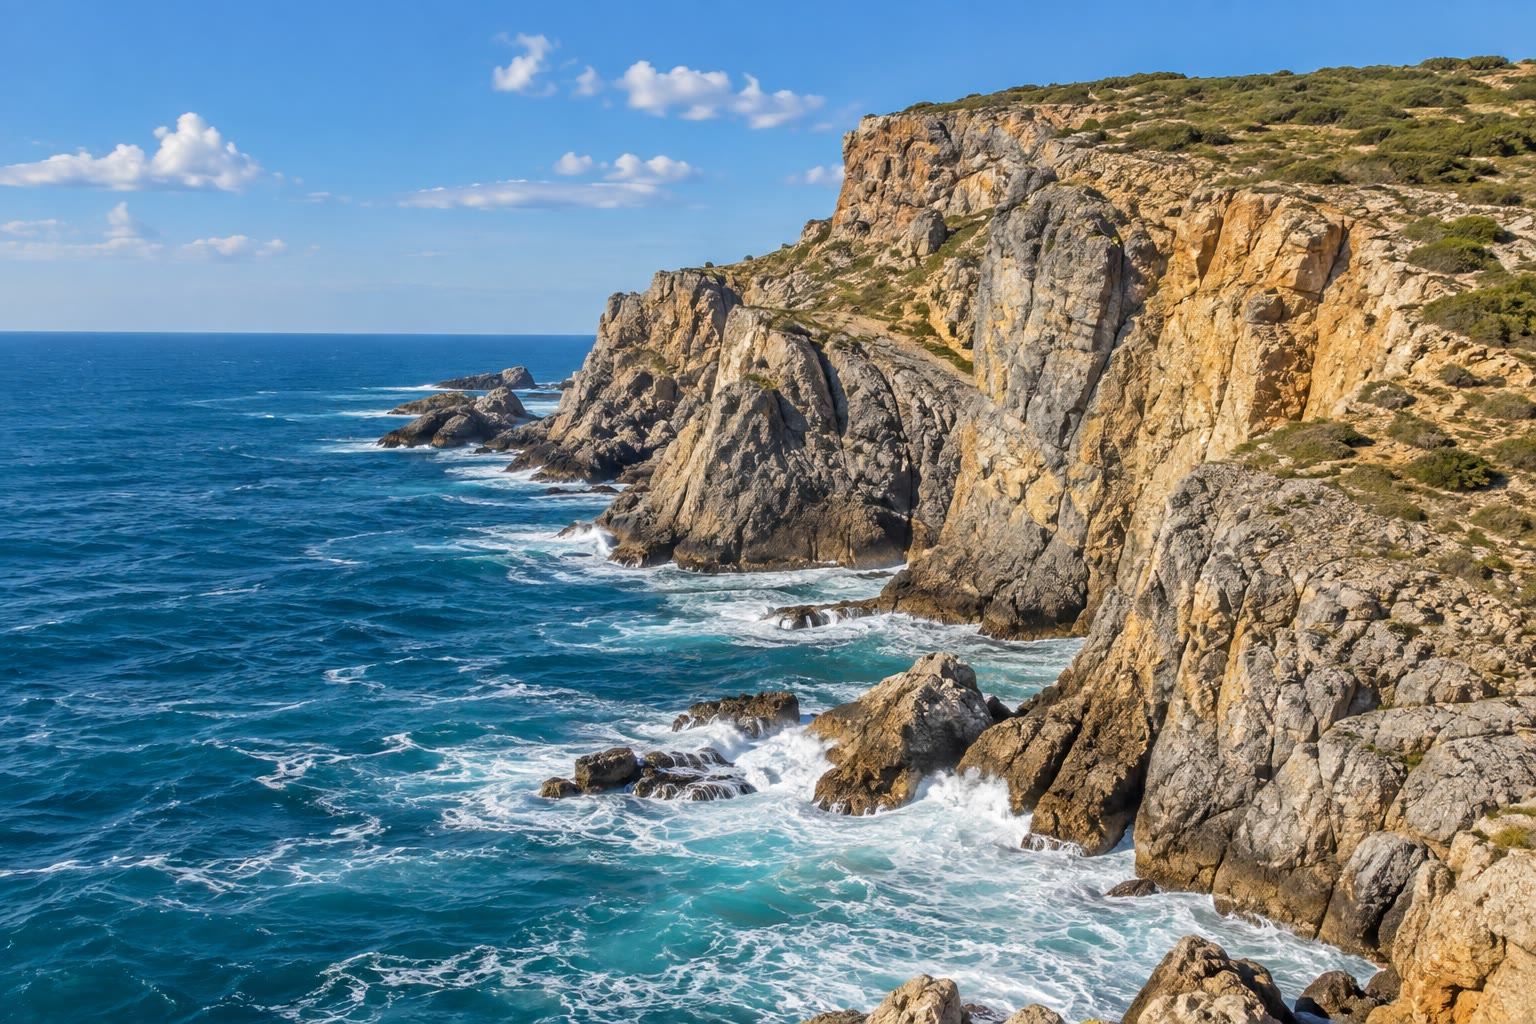
\includegraphics[width=0.55\linewidth]{images/book1/ai/g9-coastal-cliff.jpg}

{\small Gesteente, zee en \omterm{def:g4:air-a-mixture-of-gases:air}{lucht}: drie heel verschillende \omterm{def:g6:pure-substances-and-mixtures:mixture}{mengsels} van
dezelfde elementen.}
\end{omfigure}

\section{Oefeningen}

\begin{exercise}[$\star$]\label{exo:g9:elements-universe-earth:1}
Uit welke twee elementen bestaat de zon bijna helemaal?
\end{exercise}

\begin{exercise}[$\star$]\label{exo:g9:elements-universe-earth:2}
Welk element komt het meest voor in de aardkorst? En in het menselijk
lichaam (in massa)?
\end{exercise}

\begin{exercise}[$\star$]\label{exo:g9:elements-universe-earth:3}
Waar zijn de meeste elementen gemaakt die zwaarder zijn dan helium?
\end{exercise}

\begin{exercise}[$\star$]\label{exo:g9:elements-universe-earth:4}
Welk percentage van de massa van zeewater is opgelost zout?
\end{exercise}

\begin{exercise}[$\star\star$]\label{exo:g9:elements-universe-earth:5}
Tel met het diagram van de aardkorst de aandelen van zuurstof en
silicium op. Welk deel van de aardkorst is dat ongeveer?
\end{exercise}

\begin{exercise}[$\star\star$]\label{exo:g9:elements-universe-earth:6}
Waarom zit er zo weinig waterstof en helium in de aardkorst, terwijl de
zon er bijna helemaal uit bestaat?
\end{exercise}

\begin{exercise}[$\star\star$]\label{exo:g9:elements-universe-earth:7}
Hoeveel koolstof zit er in een lichaam van \qty{70}{kg} dat voor
\qty{23}{\percent} uit koolstof bestaat?
\end{exercise}

\begin{exercise}[$\star\star$]\label{exo:g9:elements-universe-earth:8}
Waarom is zuurstof in massa het meest voorkomende element van het
lichaam, terwijl waterstof dat is in aantal \omterm{def:g7:atoms-and-molecules:atom}{atomen}?
\end{exercise}

\begin{exercise}[$\star\star$]\label{exo:g9:elements-universe-earth:9}
Een blok graniet van \qty{1000}{kg} is een typisch stuk aardkorst.
Hoeveel aluminium bevat het ongeveer, volgens het diagram?
\end{exercise}

\begin{exercise}[$\star\star$]\label{exo:g9:elements-universe-earth:10}
Welke elementen staan zowel bij de belangrijkste elementen van de
aardkorst als bij die van het menselijk lichaam?
\end{exercise}

\begin{exercise}[$\star\star\star$]\label{exo:g9:elements-universe-earth:11}
Een lichaam van \qty{70}{kg} bevat ongeveer \qty{1.06}{kg} calcium.
Bereken de massa van één calciumatoom ($A = 40$), en daarna het aantal
calciumatomen. Schrijf het in wetenschappelijke notatie.
\end{exercise}

\begin{exercise}[$\star\star\star$]\label{exo:g9:elements-universe-earth:12}
De \omterm{def:g7:atoms-and-molecules:atom}{atomen} van je lichaam zijn allemaal al eerder deel geweest van iets
anders. Leg met de reis van een koolstofatoom uit waarom het totale
aantal koolstofatomen op aarde nauwelijks verandert.
\end{exercise}

\section{Probleem: Uit hoeveel atomen besta ik?}

\begin{problem}[{Weekendprobleem --- van een abundantiediagram naar het
aantal zuurstofatomen in een menselijk lichaam}]
\label{pb:g9:elements-universe-earth:1}
% ledger: body:atoms-O, body:atoms-total
Een slanke volwassene van \qty{70}{kg} bestaat in massa voor ongeveer
\qty{61}{\percent} uit zuurstof, \qty{23}{\percent} uit koolstof en
\qty{10}{\percent} uit waterstof. Neem voor de massa van een \omterm{def:g9:inside-the-atom:proton}{nucleon}
\qty{1.67e-27}{kg}; een zuurstofatoom heeft 16 \omterm{def:g9:inside-the-atom:proton}{nucleonen}, een
koolstofatoom 12, een waterstofatoom 1. De \omterm{def:g9:inside-the-atom:nucleus}{elektronen} worden
verwaarloosd.

\medskip
\noindent\textbf{Deel I --- De massa's.}
\begin{enumerate}
  \item Bereken de massa zuurstof in het lichaam.
  \item Bereken de massa koolstof en die van waterstof.
  \item Welk percentage van de massa vormen deze drie elementen samen?
  \item Het meeste van deze zuurstof en waterstof zit in één verbinding.
        Welke?
\end{enumerate}

\medskip
\noindent\textbf{Deel II --- Eén \omterm{def:g7:atoms-and-molecules:atom}{atoom}.}
\begin{enumerate}[resume]
  \item Bereken de massa van één zuurstofatoom.
  \item Bereken de massa van één koolstofatoom en van één
        waterstofatoom.
  \item Hoeveel waterstofatomen wegen samen evenveel als één
        zuurstofatoom?
  \item Waarom mag je de \omterm{def:g9:inside-the-atom:nucleus}{elektronen} verwaarlozen?
\end{enumerate}

\medskip
\noindent\textbf{Deel III --- De telling.}
\begin{enumerate}[resume]
  \item Bereken het aantal waterstofatomen in het lichaam.
  \item Bereken het aantal koolstofatomen.
  \item Bereken het aantal zuurstofatomen in het lichaam.
  \item Een zorgvuldige schatting geeft $1.61 \times 10^{27}$
        zuurstofatomen in zo'n lichaam. Vergelijk met jouw telling, en
        geef het aantal zuurstofatomen in een lichaam van \qty{70}{kg}
        in twee significante cijfers.
\end{enumerate}
\end{problem}
